% Author: Samo Fortuna
\documentclass{minimal}
\usepackage{tikz,units,amsmath}
\usetikzlibrary{arrows,positioning} 
\tikzset{
    %Define standard arrow tip
    >=stealth',
    %Define style for boxes
    center-style/.style={
           rectangle,
           draw=black, very thick,
           text width=4cm,
		   inner sep=10pt,
           minimum height=2em,
           text centered},
    bignode/.style={
           rectangle,
           rounded corners,
           draw=black, very thick,
           text width=6cm,
           inner sep=10pt,
           minimum height=2em,
           text centered},
    % Define arrow style
    pil/.style={
           <->,
           thick,
           shorten <=2pt,
           shorten >=2pt,}
}

%%% remove space above \begin{align*}
\setlength{\abovedisplayskip}{0pt}

\begin{document}

\begin{align*} 
	e_i(t) = NA\omega B(t) \\
	E_i = 4,44Nf\hat{\Phi} 						&& sin \\
	E_i = 4Nf\hat{\Phi} 						&& square \\
\end{align*}
\begin{align*} 
	L_{22} = \left(\frac{N_1}{N_2}\right)^2 \cdot L_{12} \\
	X_L=\omega L \\
	L=\frac{\Psi}{i}=\frac{N\Phi}{i}=\frac{N^2}{R_m} 	&& [\unit{Vs/A}]  \\
	R_m=\frac{l}{\mu_0\mu_rA} 			&& [\unit{A/Vs}]
\end{align*}

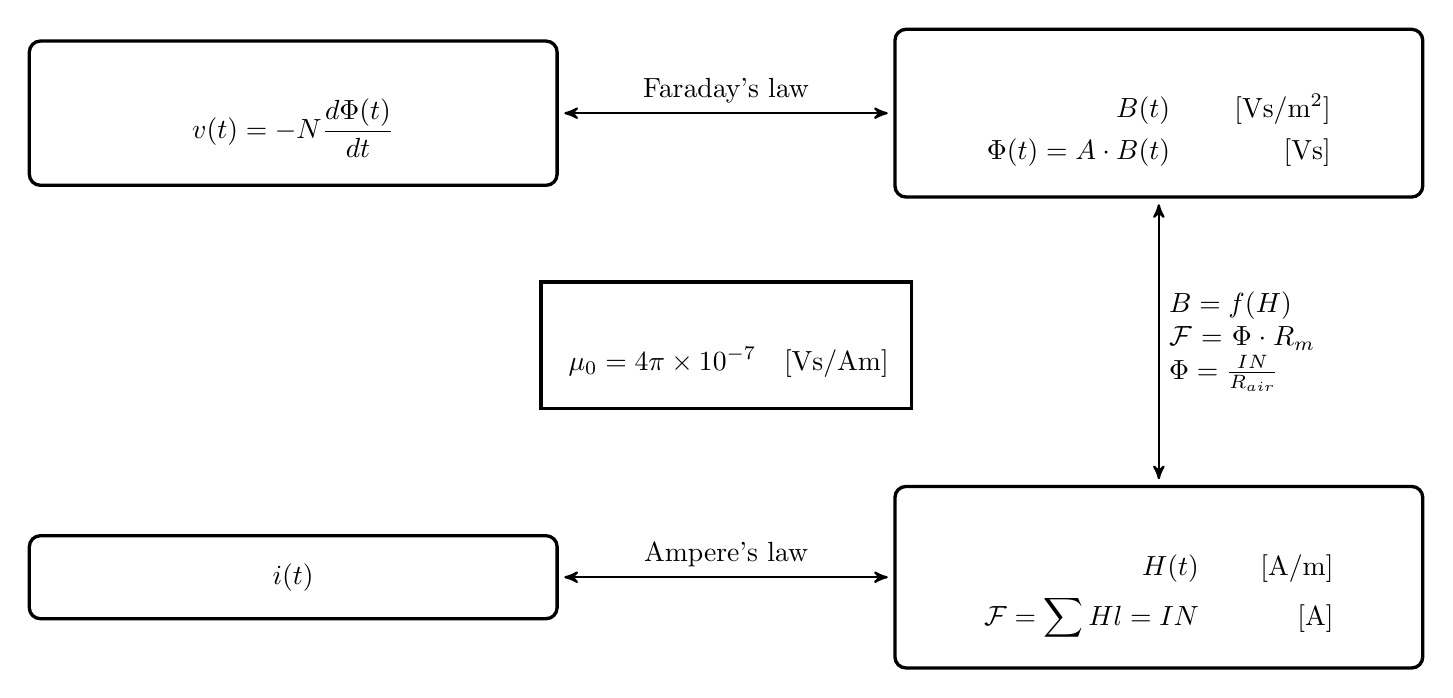
\begin{tikzpicture}[node distance=2cm, auto,]
 \node[bignode] (current) { $i(t)$ };

 \node[right=of current] (ampere) {};
 
 \node[center-style, above=of ampere] (permeability) { 
 	\begin{align*} 
 		\mu_0 = 4 \pi \times 10^{-7} && [\unit{Vs/Am}] 
 	\end{align*} 	
 };
 
 \node[bignode, right=of ampere] (mmf) { 
 	\begin{align*} 
 		H(t) && [\unit{A/m}]\\
		\mathcal{F} = \sum{Hl} = IN && [\unit{A}] 			
 	\end{align*}
  }
   	edge[pil] node[above] {Ampere's law} (current.east)  ;
  
 \node[above=of permeability] (faraday) {};
 
 \node[bignode,left=of faraday] (voltage) { 
 	\begin{align*} 
 		v(t) = -N\frac{d\Phi(t)}{dt}
 	\end{align*}
 };
 \node[bignode,right=of faraday] (flux) {
 		\begin{align*} 
 			B(t) 					&& [\unit{Vs/m^2}] \\
	 		\Phi(t)=A\cdot B(t) 	&& [\unit{Vs}]
		 \end{align*}
 	}
 	edge[pil] node[above] {Faraday's law} (voltage.east) 
 	edge[pil] node[right,text width=2cm] (BH) { 
 		$B=f(H)$\\
 		$\mathcal{F}=\Phi \cdot R_m$
 		$\Phi=\frac{IN}{R_{air}}$
 	} (mmf.north);

\end{tikzpicture}

\begin{align*} 
	X_C=-\frac{1}{\omega C} 
\end{align*}

\end{document}

%%% Local Variables:
%%% mode: latex
%%% TeX-master: t
%%% End: